%======================================================================
\section{Pair areas}\label{sec:pair-areas}
%======================================================================

We now bring together two of the $2^N$ lamps supported on the first $N$ points of ray~$1$. Their transport words are products of the $\tau_i$,
and the two configurations differ by a configuration that at most $N$ transvections clear down to a single point, where the commutator of the
two lamps is a local filling. Clearing naively would let the translation word grow; we keep it normalized after every step, so that it never
has more than $N$ factors, and each step costs $O(N)$ local fillings.

\paragraph{A worked example.} Let $N=3$ and take the lamps at $u=\{1,3\}$ and $w=\{2\}$, with transport words $T_u=\tau_1\tau_3$ and
$T_w=\tau_2$. Figure~\ref{fig:clearing} draws the clearing. Translations commute, so the commutator of the two lamps is $T_u[x,ZyZ^{-1}]T_u^{-1}$
with $Z=T_u^{-1}T_w=\tau_3^{-1}\tau_1^{-1}\tau_2$, and two relations \textsf{Q} and two swaps turn $Z$ into $T_{u_0}=\tau_1\tau_2\tau_3$, where
$u_0=u+w=\{1,2,3\}$. Choose the point $3$ of $u_0$ as the \emph{pivot}, into which the other points are cleared. The transvection $X_{13}$ adds
the value at $3$ into $1$. Conjugating $T_{u_0}$ by it leaves $\tau_1$ and $\tau_2$ alone and turns $\tau_3$ into $\tau_1\tau_3$; one swap brings
the new $\tau_1$ next to the old one, and one relation \textsf{Q} cancels them, leaving $\tau_2\tau_3$. Then $X_{23}$ turns $\tau_2\tau_3$ into
$\tau_3$ in the same way. Conjugating by $G=X_{23}X_{13}$ therefore carries the lamp at $u_0$ to the lamp at $e_3$, while $G$ is linear and
commutes with the lamp at $0$. What is left is $[x,\tau_3y\tau_3^{-1}]$, a local filling. Every identity used involves at most three points, so
Lemma~\ref{lem:local-filling} prices each of them at $L(3)$.

\begin{figure}[ht]
\centering
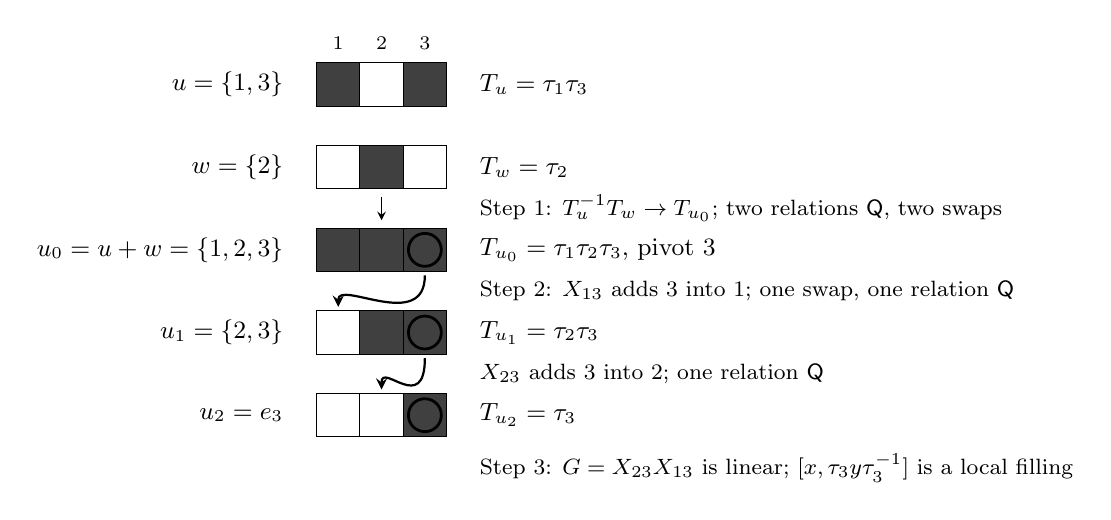
\begin{tikzpicture}[x=1cm,y=1cm,>=stealth]
\def\cw{0.55}   % cell width
\def\rh{1.05}   % row height
% a row of three cells at height #1, lit pattern #2#3#4 (1 = lit), ringed pivot column #5 (0 = none)
\newcommand{\cellrow}[5]{%
  \foreach \c/\lit in {1/#2,2/#3,3/#4}{%
    \ifnum\lit=1 \fill[black!75] ({(\c-1)*\cw},#1) rectangle ({\c*\cw},{#1+\cw}); \fi
    \draw ({(\c-1)*\cw},#1) rectangle ({\c*\cw},{#1+\cw});
  }%
  \ifnum#5>0 \draw[line width=1pt] ({(#5-0.5)*\cw},{#1+0.5*\cw}) circle ({0.38*\cw}); \fi
}
% column headers: the points 1, 2, 3 of ray 1
\foreach \c in {1,2,3}{\node[font=\scriptsize] at ({(\c-0.5)*\cw},{5*\rh+\cw+0.25}) {$\c$};}
% the two lamps
\cellrow{5*\rh}{1}{0}{1}{0}
\node[anchor=east,font=\small] at (-0.3,{5*\rh+0.5*\cw}) {$u=\{1,3\}$};
\node[anchor=west,font=\small] at ({3*\cw+0.3},{5*\rh+0.5*\cw}) {$T_u=\tau_1\tau_3$};
\cellrow{4*\rh}{0}{1}{0}{0}
\node[anchor=east,font=\small] at (-0.3,{4*\rh+0.5*\cw}) {$w=\{2\}$};
\node[anchor=west,font=\small] at ({3*\cw+0.3},{4*\rh+0.5*\cw}) {$T_w=\tau_2$};
% step 1: one translation word
\draw[->] ({1.5*\cw},{4*\rh-0.1}) -- ({1.5*\cw},{3*\rh+\cw+0.1});
\node[anchor=west,font=\footnotesize] at ({3*\cw+0.3},{3.5*\rh+0.5*\cw}) {Step 1: $T_u^{-1}T_w\to T_{u_0}$; two relations \textsf{Q}, two swaps};
\cellrow{3*\rh}{1}{1}{1}{3}
\node[anchor=east,font=\small] at (-0.3,{3*\rh+0.5*\cw}) {$u_0=u+w=\{1,2,3\}$};
\node[anchor=west,font=\small] at ({3*\cw+0.3},{3*\rh+0.5*\cw}) {$T_{u_0}=\tau_1\tau_2\tau_3$, pivot $3$};
% step 2, first transvection: from the pivot of row u_0 into cell 1 of row u_1
\draw[->,thick] ({2.5*\cw},{3*\rh-0.05}) .. controls ({2.5*\cw},{2*\rh+0.5*\cw}) and ({0.5*\cw},{3*\rh-0.1}) .. ({0.5*\cw},{2*\rh+\cw+0.05});
\node[anchor=west,font=\footnotesize] at ({3*\cw+0.3},{2.5*\rh+0.5*\cw}) {Step 2: $X_{13}$ adds $3$ into $1$; one swap, one relation \textsf{Q}};
\cellrow{2*\rh}{0}{1}{1}{3}
\node[anchor=east,font=\small] at (-0.3,{2*\rh+0.5*\cw}) {$u_1=\{2,3\}$};
\node[anchor=west,font=\small] at ({3*\cw+0.3},{2*\rh+0.5*\cw}) {$T_{u_1}=\tau_2\tau_3$};
% step 2, second transvection: from the pivot of row u_1 into cell 2 of row u_2
\draw[->,thick] ({2.5*\cw},{2*\rh-0.05}) .. controls ({2.5*\cw},{1*\rh+0.5*\cw}) and ({1.5*\cw},{2*\rh-0.1}) .. ({1.5*\cw},{1*\rh+\cw+0.05});
\node[anchor=west,font=\footnotesize] at ({3*\cw+0.3},{1.5*\rh+0.5*\cw}) {$X_{23}$ adds $3$ into $2$; one relation \textsf{Q}};
\cellrow{1*\rh}{0}{0}{1}{3}
\node[anchor=east,font=\small] at (-0.3,{1*\rh+0.5*\cw}) {$u_2=e_3$};
\node[anchor=west,font=\small] at ({3*\cw+0.3},{1*\rh+0.5*\cw}) {$T_{u_2}=\tau_3$};
% step 3
\node[anchor=west,font=\footnotesize] at ({3*\cw+0.3},{0.5*\rh+0.5*\cw-0.15}) {Step 3: $G=X_{23}X_{13}$ is linear; $[x,\tau_3y\tau_3^{-1}]$ is a local filling};
\end{tikzpicture}
\caption{The clearing of the worked example, $N=3$: the lit cells are the support of a configuration on the points $1,2,3$ of ray~$1$, the ringed
cell is the pivot, and each arrow is a transvection that adds the value at the pivot into the cell it points to. After $X_{13}$ and $X_{23}$ the
configuration $u_0=\{1,2,3\}$ has become $e_3$, and the translation word has been renormalized after each step.}
\label{fig:clearing}
\end{figure}


\begin{theorem}[Pair areas]\label{thm:pair-area}
Let $N\ge1$ and $n=\max(3,N)$. For a configuration $u$ supported in the first $N$ points of ray~$1$ let $T_u=\tau_{i_1}\cdots\tau_{i_m}$,
where $i_1<\dots<i_m$ are the points of the support of $u$. Then $T_u$ represents $\tau_u$, so $T_uaT_u^{-1}$ and $T_ubT_u^{-1}$ generate the copy
of $S_3$ at $u$; $|T_u|\le21Nn$; and for distinct such $u,w$ and $x,y\in\{a,b\}$, with $b$ the word $ac^4$,
\[
\Area_R\bigl([T_uxT_u^{-1},\,T_wyT_w^{-1}]\bigr)\ \le\ \Lambda_N:=20N^2L(n)\ \le\ C_0N^2\bigl(\delta_H(C_0N)+N\bigr)
\]
with $C_0=4.5\cdot10^4$. Consequently there are absolute constants $K'$ and $C'$ with
\[
\Lambda_N\le e^{K'N}\qquad\text{and}\qquad \Lambda_N\le C'N^{2+p_H}\qquad(N\ge1),\qquad p_H=\log107+4 .
\]
\end{theorem}

\begin{proof}
Translations commute, so $T_u$ represents $\tau_u$, and $|T_u|\le N(2\cdot10n+1)\le21Nn$. Write $L=L(n)$; by Lemma~\ref{lem:local-filling},
each of its four local identities has area at most $L$.

\emph{Step 1: one translation word.} Freely, $[T_uxT_u^{-1},T_wyT_w^{-1}]=T_u[x,ZyZ^{-1}]T_u^{-1}$ with $Z=T_u^{-1}T_w$. Replace each of the at
most $N$ factors $\tau_i^{-1}$ of $T_u^{-1}$ by $\tau_i$, at one relation \textsf{Q} each. Sort the resulting product of at most $2N$ factors
$\tau_i$ into increasing order; this takes at most $\binom{2N}2$ swaps of adjacent distinct factors, each a local filling of
Lemma~\ref{lem:local-filling}(a). Cancel the at most $N$ adjacent equal pairs, again at one relation \textsf{Q} each. The result is $T_{u_0}$ with
$u_0=u+w\ne0$, and $\Area_R(ZT_{u_0}^{-1})\le2N+N(2N-1)L\le2N^2L$. Since $Z^{\pm1}$ occurs four times in $[x,ZyZ^{-1}]$,
\[
\Area_R\bigl([T_uxT_u^{-1},T_wyT_w^{-1}]\bigr)\le8N^2L+\Area_R\bigl([x,T_{u_0}yT_{u_0}^{-1}]\bigr).
\]

\emph{Step 2: normalized clearing.} Let $s\le N$ be the size of the support of $u_0$, choose a point $j$ in it as the pivot, and list the other
points of the support as $i_1,\dots,i_{s-1}$. Put $G_l=X_{i_lj}\cdots X_{i_1j}$ and $u_l=u_0+e_{i_1}+\dots+e_{i_l}$, whose support is that of $u_0$
with $i_1,\dots,i_l$ removed; it still contains $j$, and $u_{s-1}=e_j$. We claim
\[
\Area_R\bigl(G_lT_{u_0}G_l^{-1}\,T_{u_l}^{-1}\bigr)\le2lsL\qquad(0\le l\le s-1).
\]
For $l=0$ there is nothing to prove. Given the claim for $l$, write $X=X_{i_{l+1}j}$ and $i=i_{l+1}$. Freely
$G_{l+1}T_{u_0}G_{l+1}^{-1}=X(G_lT_{u_0}G_l^{-1})X^{-1}$, which differs from $XT_{u_l}X^{-1}$ by a conjugate of a word of area at most $2lsL$. Next,
$XT_{u_l}X^{-1}$ is freely the product of the words $X\tau_{i'}X^{-1}$ over the support of $u_l$, in order. By Lemma~\ref{lem:local-filling}(b),
at a cost of at most $sL$, each of these becomes $\tau_{i'}$, except that $X\tau_jX^{-1}$ becomes $\tau_j\tau_i$. The new factor $\tau_i$ has a
partner $\tau_i$ in $T_{u_l}$, because $i$ lies in the support of $u_l$; at most $s-1$ swaps (Lemma~\ref{lem:local-filling}(a)) make the two
adjacent, and one relation \textsf{Q} cancels them. What remains is $T_{u_{l+1}}$. This step costs at most $sL+(s-1)L+1\le2sL$, which proves the
claim. The translation word is renormalized after every transvection and never has more than $s\le N$ factors.

\emph{Step 3: a single point.} Let $G=G_{s-1}$ and let $M=GT_{u_0}G^{-1}\tau_j^{-1}$, which has area at most $2s(s-1)L\le2N^2L$ by Step~2. Freely
$T_{u_0}=G^{-1}M\tau_jG$. Substituting this into the four occurrences of $T_{u_0}^{\pm1}$ in $[x,T_{u_0}yT_{u_0}^{-1}]$ and deleting the four
occurrences of $M^{\pm1}$ costs at most $8N^2L$. By Lemma~\ref{lem:local-filling}(c), $\Area_R([G,z])\le(s-1)(40n+1)$ for $z\in\{a,b\}$, and the
same bound holds for $[G,z^{-1}]$ and $[z,G^{-1}]$. Moving $y^{\pm1}$ across $G$ and $G^{-1}$, and then $x^{\pm1}$, leaves
$G^{-1}[x,\tau_jy\tau_j^{-1}]G$, at a cost of at most $4(s-1)(40n+1)$; and $[x,\tau_jy\tau_j^{-1}]$ has area at most $40n+1$ by
Lemma~\ref{lem:local-filling}(d). Altogether, since $L\ge700n$,
\[
\Area_R\bigl([x,T_{u_0}yT_{u_0}^{-1}]\bigr)\le8N^2L+4N(40n+1)+40n+1\le9N^2L,
\]
and with Step~1 the area is at most $17N^2L\le\Lambda_N$.

\emph{Growth.} Since $n\le3N$, $L(n)\le10\delta_H(4500N)+2100N$, which gives the first bound on $\Lambda_N$. With Proposition~\ref{prop:dehn}(a)
it is at most $e^{K'N}$ for a suitable $K'$. With Proposition~\ref{prop:dehn}(b) it is at most $C_0N^2(C(C_0N)^{p_H}+N)\le C'N^{2+p_H}$, since $p_H>1$.
\end{proof}

The factor $N^2$ counts local moves: at most $N$ transvections, each followed by at most $N$ commutations. The Dehn function of $H$ enters
through the local fillings, at the scale $N$ of the transport. Theorem~\ref{thm:pair-area} is the only transport input of the paper: the lower
bounds of Theorem~A (Section~\ref{sec:profile}) and of Theorem~B (Section~\ref{sec:lamp-channel}) feed it into the criterion and into the
one-round theorem.
